\newif\ifENG
\ENGtrue % 英語版を使用する場合はtrue、和文版を使用する場合はfalseに設定

\newif\ifhidejson
\hidejsontrue % JSONを表示しない場合はtrue、表示しない場合は
\hidejsonfalse % JSONを表示する場合はtrue、表示しない場合はfalseに設定

\newif\ifshowIntro
\showIntrofalse 
\showIntrotrue 

\newif\ifshowConclusion
\showConclusionfalse
\showConclusiontrue

\newif\ifshowBG
\showBGfalse 
\showBGtrue 

\newif\ifshowjson
\showjsontrue % JSONを表示する場合はtrue、表示しない場合はfalseに設定
\showjsonfalse % JSONを表示しない場合はtrue、表示しない場合はfalseに設定

\documentclass{article}
\usepackage{graphicx}
\usepackage[paperwidth=84.1cm, paperheight=118.9cm, margin=0cm]{geometry}
\usepackage{tikz}
\usepackage{hyperref}
\usepackage{fontspec}
\usetikzlibrary{positioning,shapes.callouts}% 吹き出し用
\usepackage{listings}
\usepackage{xcolor}

% JSON 用スタイル定義
\lstdefinelanguage{json}{
  basicstyle=\fontsize{26}{26}\selectfont\ttfamily,
}

\lstset{
  breaklines=true,
  basicstyle=\fontsize{26}{26}\selectfont\ttfamily,
  breakatwhitespace=false,
  breakindent=2em,
  columns=flexible,
  escapeinside={(*@}{@*)}
}

%\lstset{
%  basicstyle=\fontsize{28}{18}\selectfont\ttfamily,
%  breaklines=true,
%  columns=fullflexible,
%  escapeinside={(*@}{@*)} % 中でLaTeXを使うための逃げ
%}

% 色の定義
\definecolor{mydeepblue}{HTML}{332E83}

% カスタム色定義(例:薄いクリーム色)
\definecolor{cream}{RGB}{255, 254, 250}

% 背景用
\definecolor{deepBackground}{HTML}{332E83} % 深い藍(背景など)
\definecolor{softGray}{HTML}{CCCCCC}       % 淡い灰色(背景補助)
\definecolor{lightIvory}{HTML}{F8F5E1}     % 生成的な淡ベージュ

% タイトル・見出し用
\definecolor{katanoPurple}{HTML}{4B0082}   % 目立つ紫
\definecolor{katanoBlue}{HTML}{4466CC}     % 明るい青
\definecolor{katanoIndigo}{HTML}{3A4F92}   % 落ち着いた藍
\definecolor{katanoBrown}{HTML}{5C4033}    % 和風の焦げ茶

\definecolor{katanoMediumOrchid}{HTML}{BA55D3} % 明るい紫、ピンクがかる
\definecolor{katanoMediumPurple}{HTML}{9370DB} % 少し青みが強い
\definecolor{katanoOrchid}{HTML}{DA70D6}       % さらに明るいピンク寄り
\definecolor{katanoViolet}{HTML}{EE82EE}       % 淡い紫、明度が高い
\definecolor{katanoSlateBlue}{HTML}{6A5ACD} % くっきりめ紫
\definecolor{katanoPurpleStrong}{HTML}{6A5ACD} % SlateBlue系


\definecolor{katanoSlateBlue}{HTML}{6A5ACD} % 青紫・視認性良好
\definecolor{katanoMediumSlateBlue}{HTML}{7B68EE} % やや明るい青紫
\definecolor{katanoBlueViolet}{HTML}{8A2BE2} % かなり青い鮮やか紫

% 本文用
\definecolor{katanoTextGray}{HTML}{333333} % 濃い灰(本文)

\setmainfont{Noto Sans}
\newfontfamily\jpfont{Noto Sans Mono CJK JP}

%\setmainfont{Noto Sans CJK JP} % 日本語フォントを指定

\pagestyle{empty}

\begin{document}

\begin{tikzpicture}[remember picture, overlay]

% 背景色
%\fill[blue] (current page.south west) rectangle (current page.north east);

% 背景画像(使う場合コメントアウトを外す)
%\node[anchor=south west, inner sep=0] at (current page.south west) {
%  \includegraphics[width=\paperwidth,height=\paperheight]{background.jpg}
%};

% 背景画像をページ全面に敷く
\ifshowBG
\node (bg-pic) [
  anchor=south west,
  inner sep=0,
  opacity=0.2, % 透明度を設定
] at (current page.south west) {
  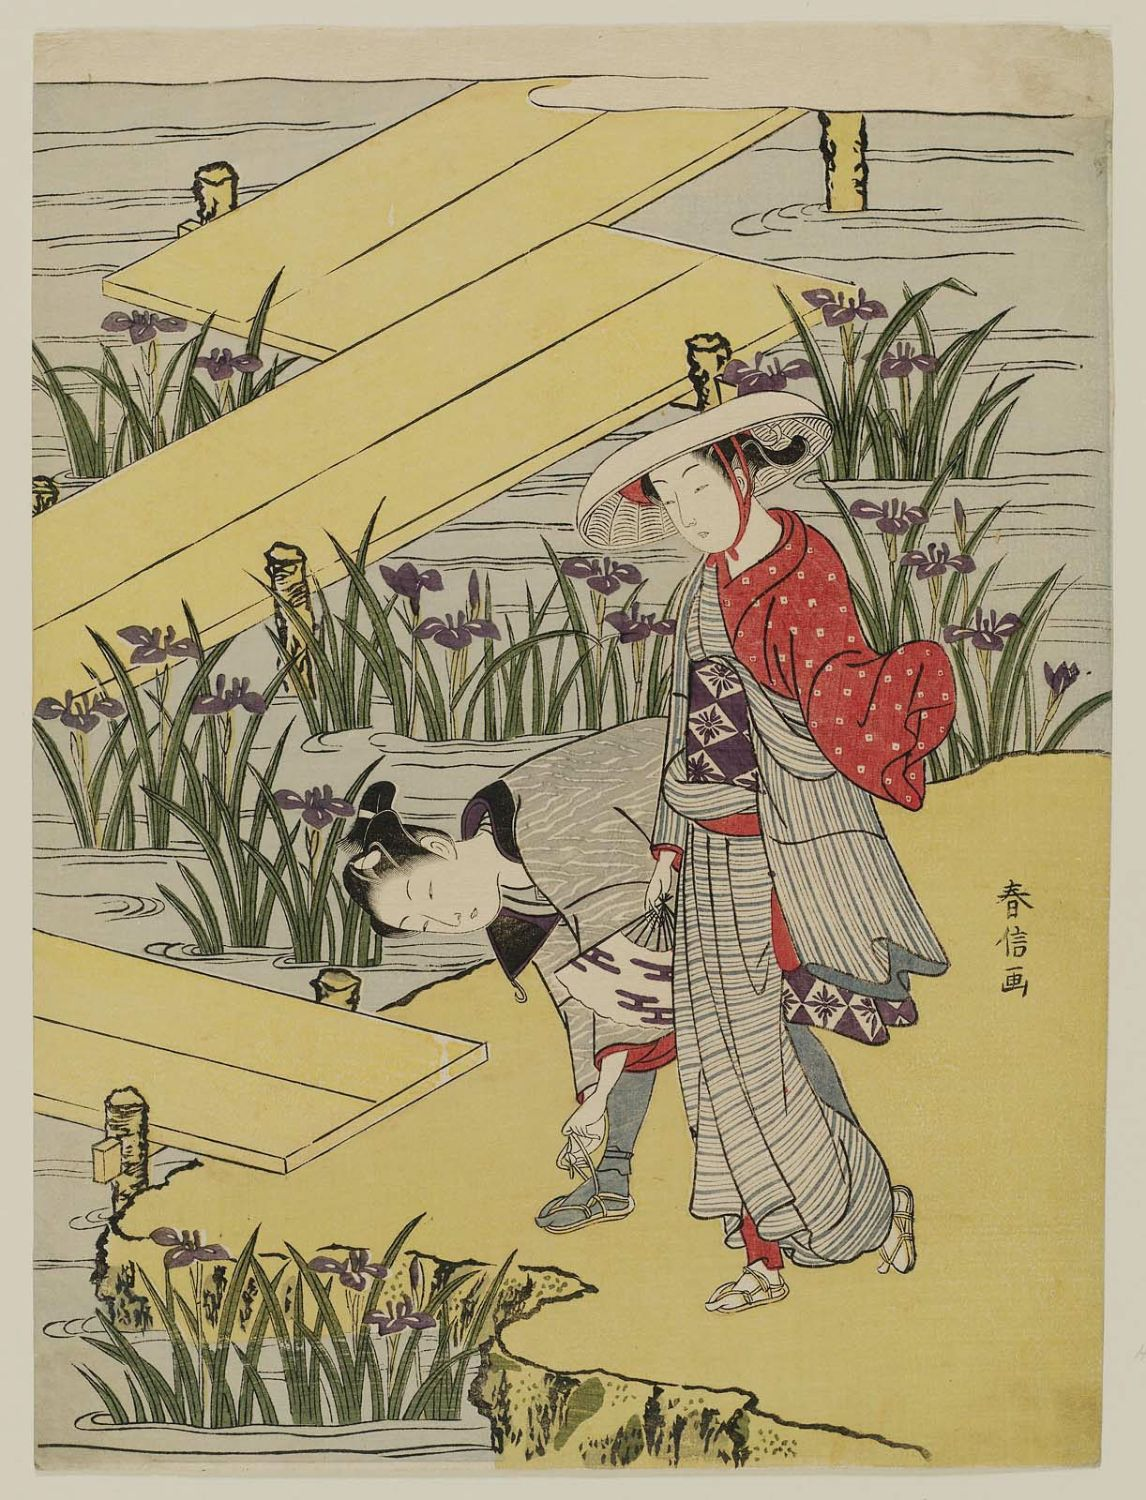
\includegraphics[width=\paperwidth,height=\paperheight]{
%  ise-katano.jpg
    images/yatsuhashi.jpg
 }
};
\fi

% 画像の著作権
\node[
  anchor=north west,
  align=left,
  color=katanoMediumPurple,
  font=\fontsize{20pt}{20pt}\bfseries
] at ([xshift=1cm,yshift=2cm]current page.south west) {
\ifENG
% Background: Katano; Admiring the Scattered Cherry Blossoms
Background Image courtesy of the Museum of Fine Arts, Boston; Public Domain
%  \jpfont{画像提供:\textbf{いせかたの}(伊勢物語のカタノ)}
\else
画像出典:ボストン美術館(パブリックドメイン)
\fi
};

% Title
\node[
  anchor=north,
  align=center,
  text=blue!80!black,
  font=\fontsize{60pt}{70pt}\bfseries
] at ([yshift=-2cm]current page.north) {
  Translating Ise Monogatari through the Lens of Process Grammar Model
};

% Subtitle
\node[
  anchor=north,
  align=center,
  text=blue!80!black,
  font=\fontsize{60pt}{70pt}\bfseries
] at ([yshift=-5cm]current page.north) {
  A Bilingual and Structured Approach to Classical Japanese Narratives
};

% Authors
\node[
  anchor=north,
  align=center,
  font=\fontsize{50pt}{40pt}\bfseries
] at ([yshift=-8cm]current page.north) {
Hilofumi Yamamoto{\raisebox{1.5ex}{\fontsize{20pt}{20pt}\selectfont 1}}
\quad
Bor Hodošček{\raisebox{1.5ex}{\fontsize{20pt}{20pt}\selectfont 2}}
\quad
Xudong Chen{\raisebox{1.5ex}{\fontsize{20pt}{20pt}\selectfont 1}}
};

% 所属
\node[
  anchor=north,
  align=center,
  font=\fontsize{40pt}{30pt}\bfseries
] at ([yshift=-11cm]current page.north) {
{\raisebox{1.5ex}{\fontsize{20pt}{20pt}\selectfont 1}}
Institute of Science Tokyo
\quad
{\raisebox{1.5ex}{\fontsize{20pt}{20pt}\selectfont 2}}
The University of Osaka
};

\ifshowIntro

% タイトルノード(上に浮かせる)
\node[
  draw=katanoBlue,
  line width=5pt,
  inner sep=10mm, 
  anchor=north west,
  text width=61cm,
  align=left,
  text=mydeepblue,
  font=\fontsize{30pt}{20pt}\bfseries
] (introbox) at ([xshift=4cm,yshift=-14cm]current page.north west) {
%  \textbf{\fontsize{40pt}{30pt}\selectfont Introduction}\\[1em]
  \textcolor{katanoBrown}{
    \begin{itemize}
      \item Ise Monogatari: A classic of Japanese literature
      \item Process Grammar Model: A framework for understanding narrative structures
      \item Bilingual approach: Bridging classical Japanese and modern English
%      \item {\jpfont 逐語訳は、原文の意味を正確に伝えることが難しい。また、原文に忠実に単語毎に訳しているので、文法的に不自然な訳文になることが多い。これが、注釈書に見られる訳文のぎこちなさの一因である。しかし、これは学術を否定すべき要素にはならない。むしろ、記録上に残されていない要素を補うために、逐語訳が必要になることもある。逐語訳は、原文の意味を正確に伝えることが難しい。また、原文に忠実に単語毎に訳しているので、文法的に不自然な訳文になることが多い。これが、注釈書に見られる訳文のぎこちなさの一因である。しかし、これは学術を否定すべき要素にはならない。}
%      \item Literal translation struggles to accurately convey the original meaning. Additionally, since it translates word-for-word faithfully to the original text, it often results in grammatically unnatural translations. This is one reason for the awkwardness found in annotated translations. However, this should not be a factor to negate academic work. Rather, literal translation may be necessary to supplement elements not recorded in the original text.
        % \item 文章読解は、まず書かれたことを忠実に拾い、再構成することから始まる。
%      \item Text comprehension begins with faithfully capturing what is written and reconstructing it.
        % \item 翻訳も現代語にしろ、英訳にしろ、まずは原文に忠実であることが重要である。
%      \item In translation, whether into modern Japanese or English, fidelity to the original text is paramount.
        % \item その上で、読み手にとって自然な文章になるように、適切な補足や解説を加えることが求められる。
%      \item On that basis, it is necessary to add appropriate supplements and explanations to make the text natural for the reader.
        % \item しかし、読み取るということには、読者の解釈が入る余地がある。
%      \item However, interpretation by the reader leaves room for subjective understanding.
        % \item その解釈を翻訳に反映させることは、学術的な翻訳としては避けるべきである。
%      \item Reflecting that interpretation in the translation should be avoided in academic translations.
        % \item なぜならば、1. 原文に書かれていないことを、翻訳者の解釈で補うことは、原文の意味を歪める可能性があるからである。2. 読者が翻訳を通じて、原文の意味を推測することができなくなるからである。3. そのような翻訳は、原文を読むことによる楽しみを損なうからである。
%      \item This is because: 1. Supplementing the original text with the translator's interpretation can distort the original meaning. 2. Readers may be unable to infer the original meaning through the translation. 3. Such translations diminish the enjoyment of reading the original text.
        % \item 逐語訳の課題: できる限り、しかし完璧ではない。
%      \item Challenges in literal translation: as best as possible, but not perfect.
        % \item gloss の本質は「原語を知らなくても、意味と文法機能が理解できる」記述にある。
%      \item The essence of gloss is to provide a description that allows understanding of meaning and grammatical function without knowing the original language.
        % \item その上で、読者は、原文を読み解く楽しみを味わうことができるし、これを翻訳者が奪ってはならない。
%      \item On that basis, readers can enjoy deciphering the original text, and this should not be taken away by the translator.
      % \item その解釈の過程を奪わないようにするために、4段階の翻訳プロセスを▼開発した。
%      \item To avoid taking away the process of interpretation, we have developed a 4-step translation process.
        % \item その1ステップ目として、逐語訳を行う。
%      \item The first step is to perform a literal translation.
        % \item 2ステップ目として、逐語訳を基本として、句の単位に、いわば、口述順序を尊重するために、句の意味が独立して成立する単位に分割した。
%      \item The second step is to divide the literal translation into units where the meaning of phrases can stand independently, respecting the order of narration. 
        % \item 3ステップ目として、原文の言語要素にglossを付与する。glossは、原文の意味と文法機能を理解できるようにするためのものである。このgloss の付与については、句の単位で行い、他の句との関係は考慮しない。その意味で、文を前提とする句構造規則を用いることはしない。
%      \item The third step is to add gloss to the linguistic elements of the original text. Gloss is intended to help understand the meaning and grammatical function of the original text. This glossing is done at the phrase level without considering relationships with other phrases. In that sense, we do not use phrase structure rules that assume sentences.
        % \item 4ステップ目として、句と句の関係を考慮して、自然な現代語訳、あるいは英語になるように、句を組み合わせていく。このとき、原文に書かれていないことを、翻訳者の解釈で補うことは避ける。
%      \item The fourth step is to combine phrases into a natural modern Japanese or English translation, considering the relationships between phrases. At this time, we avoid supplementing the original text with the translator's interpretation.
        % \item そのようにして、原文に忠実でありながら、読み手にとって自然な翻訳を提供することを意図している。
%      \item In this way, we aim to provide a translation that is faithful to the original text while being natural for the reader.
    \end{itemize} 
  }
};

\node[
  anchor=south west,
  font=\bfseries\fontsize{40pt}{30pt}\selectfont,
  text=mydeepblue,
  fill=cream,
  inner sep=5pt
] at ([xshift=10mm, yshift=-10mm]introbox.north west) {Introduction};

\fi%ifshowIntro

%------------------------------------
 % JSON 本体 ise.json
\node[anchor=north west ] (json) at ([xshift=6cm,yshift=-22cm]current page.north west) {
\jpfont 
  \begin{minipage}{0.9\textwidth}
\ifhidejson
  "kana (roman)": "(*@\jpfont かりしありきけるにいきあひて、みちにてうまのくちをとりて、「かうかうなむおもふ」といひければ、あはれがりて、きてねにけり。 @*)",
    {
    "phrase": "(*@\jpfont 狩しありきけるに @*)",
      "gloss": "while he was out hunting",
      "words": [
        { "word": "(*@\jpfont 狩 @*)", "gloss": "hunting" },
        { "word": "(*@\jpfont し @*)", "gloss": "do.PST" },
        { "word": "(*@\jpfont ありき @*)", "gloss": "walked.about.PST" },
        { "word": "(*@\jpfont ける @*)", "gloss": "PST" },
        { "word": "(*@\jpfont に @*)", "gloss": "when" }
      ]
    },
\fi%ifhidejson
\begin{lstlisting}[language=json]
{
  "date": [20240721, 20250214, 20250508],
  "id": 6,
  "text": "(*@\jpfont 狩しありきけるにいきあひて、道にて馬の口をとりて、「かうかうなむ思ふ」といひければ、あはれがりて、来て寝にけり。 @*)",
  "kana (roman)": "karishi ari kikeru ni ikiahite, michi nite uma no kuchi wo torite, 'kaukau namu omofu' to ihikereba, aharegarite, kite ne nikeri",
  "koutei": "...",
  "honkoku": "...",
  "translation-ja": "(*@\jpfont 狩りをして歩いているときに出会って、道で馬の口をつかんで、「こうこうと思っています」と言ったので、同情して、来て寝た。 @*)",
  "translation-en": "While out hunting, he encountered [her], and on the road took hold of the horse's bridle, saying, 'This is what I think.' Feeling moved, [she] came and lay down [with him].",
  "phrase-gloss": [
    ... (omitted for brevity and bravery) ...
    {
      "phrase": "(*@\jpfont 道にて馬の口をとりて @*)",
      "gloss": "on the road took hold of the horse's bridle",
      "words": [
        { "word": "(*@\jpfont 道 @*)", "gloss": "road" },
        { "word": "(*@\jpfont にて @*)", "gloss": "LOC.CVB" },
        { "word": "(*@\jpfont 馬 @*)", "gloss": "horse" },
        { "word": "(*@\jpfont の @*)", "gloss": "GEN" },
        { "word": "(*@\jpfont 口 @*)", "gloss": "mouth / bridle" },
        { "word": "(*@\jpfont を @*)", "gloss": "ACC" },
        { "word": "(*@\jpfont とり @*)", "gloss": "take" },
        { "word": "(*@\jpfont て @*)", "gloss": "CVB" }
      ]
    },
    {
      "phrase": "(*@\jpfont 「かうかうなむ思ふ」といひければ @*)",
      "gloss": "saying, 'This is what I think'",
      "words": [
        { "word": "(*@\jpfont かうかう @*)", "gloss": "thus and thus" },
        { "word": "(*@\jpfont なむ @*)", "gloss": "FOC" },
        { "word": "(*@\jpfont 思ふ @*)", "gloss": "think" },
        { "word": "(*@\jpfont と @*)", "gloss": "QUOT" },
        { "word": "(*@\jpfont いひ @*)", "gloss": "say" },
        { "word": "(*@\jpfont けれ @*)", "gloss": "PST" },
        { "word": "(*@\jpfont ば @*)", "gloss": "when" }
      ]
    },
    {
      "phrase": "(*@\jpfont あはれがりて、来て寝にけり @*)",
      "gloss": "being moved, she came and lay with him",
      "words": [
        { "word": "(*@\jpfont あはれがり @*)", "gloss": "be.moved" },
        { "word": "(*@\jpfont て @*)", "gloss": "CONJ" },
        { "word": "(*@\jpfont 来 @*)", "gloss": "come" },
        { "word": "(*@\jpfont て @*)", "gloss": "CONJ" },
        { "word": "(*@\jpfont 寝 @*)", "gloss": "(*@\textcolor{red}{sleep} @*)" },
        { "word": "(*@\jpfont に @*)", "gloss": "PERF" },
        { "word": "(*@\jpfont けり @*)", "gloss": "PST" }
      ]
    @*)}
  ],
  "abbreviations": {
    "CONJ": "conjunctive",
    "PST": "past",
    "LOC": "locative",
    "GEN": "genitive",
    "ACC": "accusative",
    "FOC": "focus",
    "QUOT": "quotative",
    "PERF": "perfective"
  },
  "translation-ja-natural": "(*@\jpfont 男が狩りに出かけていたとき、道で出会った三男が馬の口をつかみ、「こんなふうに思っています」と伝えた。 男はそれを聞いて心を動かされ、ある女のもとへ行き、一夜を共にした。 @*)",
  "translation-en-natural": "While the man was out hunting, he met a young man on the road who took hold of his horse’s bridle and said, 'This is how I feel.' Moved by those words, the man went to a certain woman and spent the night with her.",
  "notes-ja": [....],
  "notes-en": [
    {
            "title": "The narrator and the 'man'",
            "note": "In the Ise Monogatari, the narrator refers to himself in the third person as 'the man.' This self-distancing technique allows the text to feel autobiographical while maintaining a poetic and narrative detachment. In this passage, the narrator—presumed to be Narihira—is recounting his own experience in such terms."
          },
\end{lstlisting}
  \end{minipage}
};

%=================================================
% キャラクター画像 kaukau what? presenboy01.png
\node[left=-4cm of json, yshift=2cm] (char01) {
 % 
\includegraphics[width=10cm]{images/onionboy.png}
  
\includegraphics[width=10cm]{images/presenboy01.png}
};
% 雲型吹き出し
\node[
  right=-6.5cm of char01, 
  yshift=5.6cm,
  rectangle callout,
  rounded corners=15pt, 
  callout relative pointer={(-0.3cm,-.6cm)},
%  anchor=south east,
  draw,
  fill=white,
  text width=5cm,
  align=center,
  inner sep=20pt,
  font=\fontsize{30pt}{30pt}\bfseries
  ] at (char01.east) {Thus and thus..., what?};
%--------------------------------------------------
% キャラクター画像 kaukau what? presenboy02.png
\node[left=-4cm of json, yshift=33cm] (char02) {
% % 
\includegraphics[width=10cm]{images/onionboy.png}
  \reflectbox{
\includegraphics[width=10cm]{images/presenboy02.png}}
};
% 雲型吹き出し
\node[
  right=-6.5cm of char02, 
  yshift=3.8cm,
  rectangle callout,
  rounded corners=15pt, 
  callout relative pointer={(-1.0cm,-1.0cm)},
%  anchor=south east,
  draw,
  fill=white,
  text width=8cm,
  align=center,
  inner sep=10pt,
  font=\fontsize{30pt}{30pt}\bfseries
  ] at (char02.east) {52 dan, ID 6};
%------------------------------------


% キャラクター画像 kaukau what? otto.png
\node[left=-26cm of json, yshift=-12cm] (char03) {
% % 
\includegraphics[width=10cm]{images/onionboy.png}
  \reflectbox{
\includegraphics[width=4cm]{images/otto.png}}
};
% 雲型吹き出し
\node[
  right=-6.5cm of char03, 
  yshift=3.8cm,
  rectangle callout,
  rounded corners=15pt, 
  callout relative pointer={(-1.0cm,-1.0cm)},
%  anchor=south east,
  draw,
  fill=white,
  text width=8cm,
  align=center,
  inner sep=10pt,
  font=\fontsize{30pt}{30pt}\bfseries
  ] at (char03.east) {\textcolor{red}{Sleep}? With whom?};
%------------------------------------
%==================================


\ifshowjson
% 左上テキストボックス
\node[
  draw=katanoBlue,
  line width=3pt,
  inner sep=10mm, 
  anchor=north west,
  text width=35cm,
  align=left,
  text=mydeepblue,
  font=\fontsize{30pt}{20pt}\bfseries
] at ([xshift=4cm,yshift=-27cm]current page.north west) {
  \textbf{\fontsize{40pt}{30pt}\selectfont Problem}\\[1em]
  \textcolor{katanoBrown}{
    \begin{itemize}
      \item Translation used to write unwritten elements in the original text.
      \item Translation has not been provided the intention of the author's unwritten meaning.
      \item Translation does not allow readers to speculate the author's intention.
      \item The original work would be less interesting by reading the such translation.
   \end{itemize} 
  }
};
\fi%ifshowjson

\ifshowjson
% 右上テキストボックス
\node[
  draw=katanoBlue,
  line width=3pt,
  inner sep=10mm, 
  anchor=north east,
  text width=35cm,
  align=left,
  text=mydeepblue,
%  font=\fontsize{30pt}{20pt}\bfseries
  font=\jpfont\fontsize{30pt}{20pt}\bfseries
] at ([xshift=-3cm,yshift=-15cm]current page.north east) {
  \textbf{\fontsize{40pt}{30pt}\selectfont Methods}\\[1em]
  \textcolor{katanoBrown}{
    \begin{itemize}
      \item 4-Step Translation Process
      \item Use of Process Grammar Model
%      \item gloss の本質は「原語を知らなくても、意味と文法機能が理解できる」記述にある。
      \item The essence of gloss is to provide a description that allows understanding of meaning and grammatical function without knowing the original language.
%      \item その点で、あなたの設計方針は正確で、本質を突いています。
      \item In that respect, this design philosophy is accurate and gets to the essence.
    \end{itemize} 
  }
};

\fi%ifshowjson

% ariwara no narihira ason
\node[
  draw=katanoBlue,
  line width=0pt,
  inner sep=10mm, 
  anchor=north east,
  text width=12cm,
  align=center,
  text=mydeepblue,
  font=\jpfont\fontsize{20pt}{10pt}\bfseries
] at ([xshift=-3cm,yshift=-7cm]current page.north east) {
  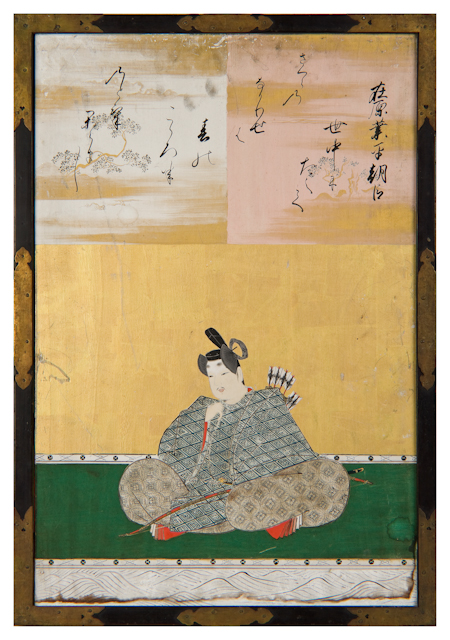
\includegraphics[trim=110 90 90 310,clip,width=12cm]{images/ariwaranonarihira.jpg}
  \\[.5em]
  \textbf{\fontsize{27pt}{10pt}\selectfont Ariwara no Narihira}
  
\includegraphics[trim=0 0 0 0,clip,width=1.2cm]{images/PD-icon.png}
};

\ifshowConclusion
% 中央下テキスト
% results and conclusion
\node[
  draw=katanoBlue,
  line width=5pt,
  inner sep=10mm, 
  anchor=north west,
  text width=75cm,
  align=left,
  text=mydeepblue,
  font=\fontsize{30pt}{20pt}\bfseries
] (conclusionbox) at ([xshift=4cm, yshift=-100cm]current page.north west) {
%  \textbf{\fontsize{40pt}{30pt}\selectfont Results and Conclusion}\\[1em]
  \textcolor{katanoBrown}{
  \begin{itemize}
    % \item 伊勢物語全125段の日英▼逐語訳と自然訳を作成した。
    \item Created a complete bilingual literal and natural translation of all 125 sections of Ise Monogatari.
      % \item プロセス文法モデルを用いて、逐語訳を句の単位に分割し、各句にglossを付与した。
    \item Using the Process Grammar Model, we segmented the literal translation into phrases and added gloss to each phrase.
      % \item その上で、句と句の関係を考慮して、自然な現代語訳、あるいは英語になるように、句を組み合わせていった。
    \item On that basis, we combined phrases into a natural modern Japanese or English translation, considering the relationships between phrases.
      % \item そのようにして、原文に忠実でありながら、読み手にとって自然な翻訳を提供することができた。
%    \item In this way, we were able to provide a translation that is faithful to the original text while being natural for the reader.
      % \item このプロセスを通じて、伊勢物語の理解が深まり、また、逐語訳と自然訳の両方を提供することで、読者が原文の意味を推測する楽しみを損なうことなく、原文の意味を正確に伝えることができた。
%    \item Enhanced understanding of Ise Monogatari
%    \item Effective bilingual translation
%    \item Insights into narrative structures
%    \item Check the flow of the translation process
      % \item 逐語訳の課題: できる限り、しかし完璧ではない。
%    \item Challenges in literal translation: as best as possible, but not perfect.
%    \item Future Work: Expanding to other classical texts such as Tosa Nikki.
      % \item 繰り返し、このプロセスを通じて、翻訳の質を向上させる。
%    \item Repeatedly improve translation quality through this process.
  \end{itemize}
  }
};
\fi%ifshowConclusion

\node[
  anchor=south west,
  font=\bfseries\fontsize{40pt}{30pt}\selectfont,
  text=mydeepblue,
  fill=cream,
  inner sep=5pt
  ] at ([xshift=10mm, yshift=-10mm]conclusionbox.north west) {Conclusion};

%\ifshowjson
% 中央下右テキスト
\node[
  draw=katanoBlue,
  line width=5pt,
  inner sep=10mm, 
  anchor=north west,
  text width=75cm,
  align=left,
  text=mydeepblue,
  font=\fontsize{30pt}{20pt}\bfseries
] (refbox) at ([xshift=4cm, yshift=-110cm]current page.north west) {
%  \textbf{\fontsize{40pt}{30pt}\selectfont References}\\[1em]
  \begin{itemize}
  \item Yamamoto, H. (2025). Process Grammar Model (v1.0.11). Zenodo. 
  \href{https://doi.org/10.5281/zenodo.15613134}{
    \texttt{https://doi.org/10.5281/zenodo.15613134}
    
\includegraphics[height=0.9cm]{images/zenodo.15613134.png}}
  \item Yamamoto, H. (2024). The Tales of Ise, Contemporary Japanese and English translation dataset (v1.0.1) [Data set]. Zenodo. 
    \href{https://doi.org/10.5281/zenodo.13994483}{
    \texttt{https://doi.org/10.5281/zenodo.13994483}
    
\includegraphics[height=0.9cm]{images/zenodo.13994483.png}}
  \end{itemize}
};

\node[
  anchor=south west,
  font=\bfseries\fontsize{40pt}{30pt}\selectfont,
  text=mydeepblue,
  fill=cream,
  inner sep=5pt
  ] at ([xshift=10mm, yshift=-10mm]refbox.north west) {References};


%\fi%ifshowjson

% ロゴ(右下)
\node[
  anchor=south east
] at ([xshift=-1cm,yshift=1cm]current page.south east) {
  
\includegraphics[height=4cm]{images/sciencetokyo.png}
  
\includegraphics[trim=30 30 30 30, clip, height=4cm]{images/theUnivOsaka.jpg}
};

\end{tikzpicture}

\end{document}



